\chapter{PYTHON}

\section{Teori}
\subsection{Sejarah python}
\par
SEJARAH PHYTON
Python dikembangkan oleh Guido van Rossum pada tahun 1990 di CWI, Amsterdam sebagai kelanjutan dari bahasa pemrograman ABC. Versi terakhir yang dikeluarkan CWI adalah 1.2.
Tahun 1995, Guido pindah ke CNRI sambil terus melanjutkan pengembangan Python. Versi terakhir yang dikeluarkan adalah 1.6. Tahun 2000, Guido dan para pengembang inti Python pindah ke BeOpen.com yang merupakan sebuah perusahaan komersial dan membentuk BeOpen PythonLabs. Python 2.0 dikeluarkan oleh BeOpen. Setelah mengeluarkan Python 2.0, Guido dan beberapa anggota tim PythonLabs pindah ke DigitalCreations.
Saat ini pengembangan Python terus dilakukan oleh sekumpulan pemrogram yang dikoordinir Guido dan Python Software Foundation. Python Software Foundation adalah sebuah organisasi non-profit yang dibentuk sebagai pemegang hak cipta intelektual Python sejak versi 2.1 dan dengan demikian mencegah Pythondimiliki oleh perusahaan komersial. Saat ini distribusi Python sudah mencapai versi 2.6.1 dan versi 3.0. Nama Python dipilih oleh Guido sebagai nama bahasa ciptaannya karena kecintaan guido pada acara televisi Monty Python's Flying Circus. Oleh karena itu seringkali ungkapan-ungkapan khas dari acara tersebut seringkali muncul dalam korespondensi antar pengguna \textit{Python.}

\subsection{Perbedaan python 2 dan 3}
\par Perbedaan phython 2 dan 3 adalah versinya , alasan kenapa tiap vers berbeda karena memang setiap produk akan terus memperbaiki dan mengoptimalkan fitur – fitur yang ada demi terwujdnya produk yang efektif kedepanya,ini lah beberapa perbedaan phython 2 dan 3
\par Pada intinya adalah bagaimana supaya python 2 mensuport versi terbaru mereka diatasnya seperti python 3.Bagaimana cara menggunakannya cukup tambahkan modul python 3 di python 2 berikut : \\
From _ future _ import division\\
selain itu juga masih ada lagi yang masih bisa digunakan di python 2 diantaranya adalah : \\
nested _ scopes # statically nested scope \\
generators # simplr generators\\
division # changing the division operator\\
absolute _ import # import: multi - line and absolute/relative \\
with _ statement # the "with" statement\\
print _ function # make print function\\
unicode _ literals # Byte literals in python 3000

\section{Instalasi}
\subsection{instalasi python 3}

\par\large Langkah - Langkah Penginstallan \textit{Anaconda}
Sebelum menginstall aplikasi \textit{Anaconda} kita harus memperhatikan versi \textit{Windows} anda apakah \textit{windows} anda 32bit atau 64bit jadi anda harus menginstall versi \textit{Anaconda} yang sesuai dengan \textit{windows} anda. 
\begin{enumerate}
\item Buka aplikasi \textit{installer Anaconda} tersebut lalu akan muncul seperti ini 

\begin{figure}[!htbp]
    \centering
    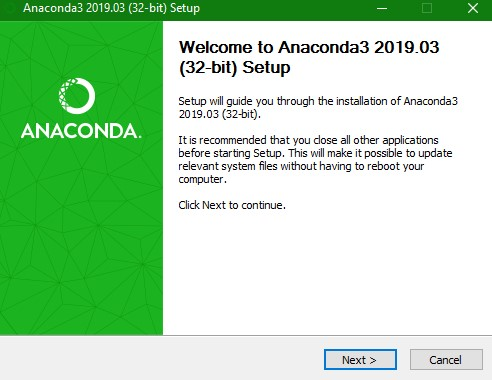
\includegraphics[scale=0.6]{gambar/1.jpg}
    \caption{\textit{Install anaconda}}
    \label{Figure1}
\end{figure}

 
\item Lalu klik next

\begin{figure}[!htbp]
    \centering
    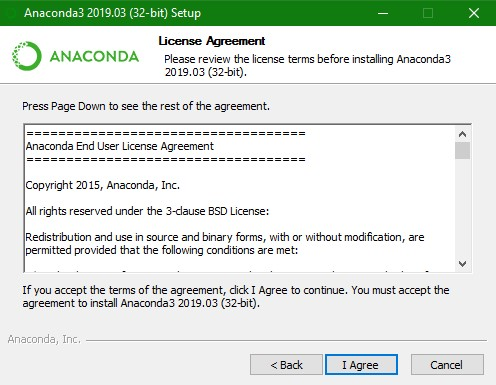
\includegraphics[scale=0.6]{gambar/2.jpg}
    \caption{\textit{Klik next pada installer anaconda}}
    \label{Figure2}
\end{figure}



\item Selanjutnya klik \textit{I Agree}

\begin{figure}[!htbp]
    \centering
    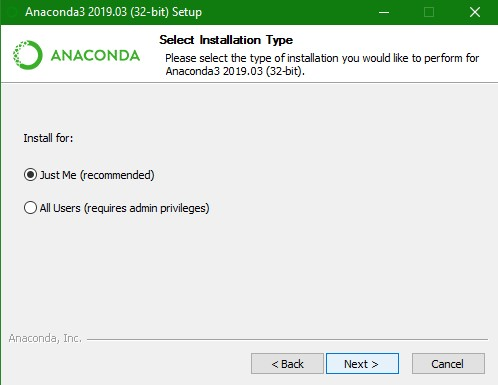
\includegraphics[scale=0.6]{gambar/3.jpg}
    \caption{\textit{Klik i agree pada installer anaconda}}
    \label{Figure3}
\end{figure}


\item Lalu pilih \textit{Just Me (recommended)} agar sesuai dengan komputer yang ada miliki

\begin{figure}[!htbp]
    \centering
    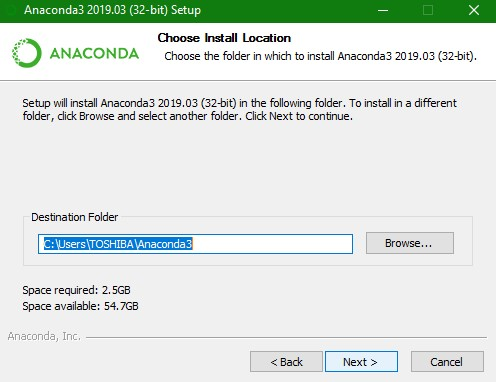
\includegraphics[scale=0.6]{gambar/4.jpg}
    \caption{\textit{Pilih just me(recommended)}}
    \label{Figure4}
\end{figure}


\item Lalu anda pilih lokasi tempat penyimpanan aplikasi tersebut

\begin{figure}[!htbp]
    \centering
    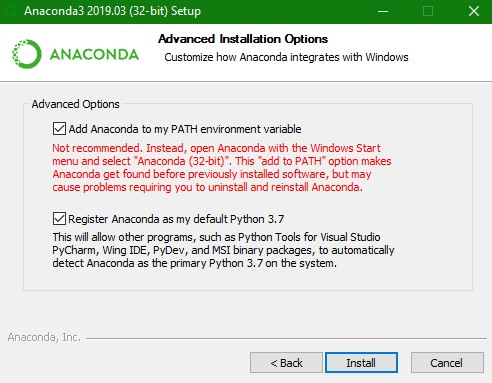
\includegraphics[scale=0.6]{gambar/5.jpg}
    \caption{\textit{Pilih lokasi penyimpanan}}
    \label{Figure5}
\end{figure}

\item Lalu anda klik \textit{add Anaconda to my path environment variable}, agar saat mengisntall \textit{selenium }langsung ke \textit{path anaconda} tidak ke aplikasi yang lain.

\begin{figure}[!htbp]
    \centering
    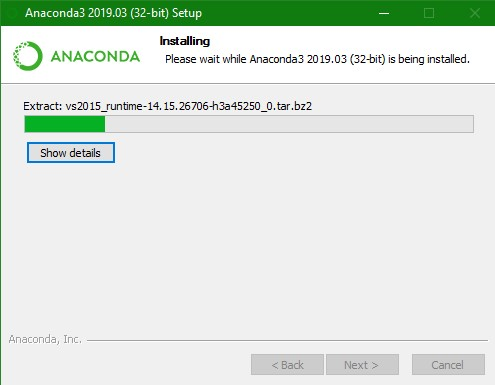
\includegraphics[scale=0.6]{gambar/6.jpg}
    \caption{\textit{Add Anaconda to my path environment variable}}
    \label{Figure6}
\end{figure}

\item Tunggu sampai instalasi selesai


\begin{figure}[!htbp]
    \centering
    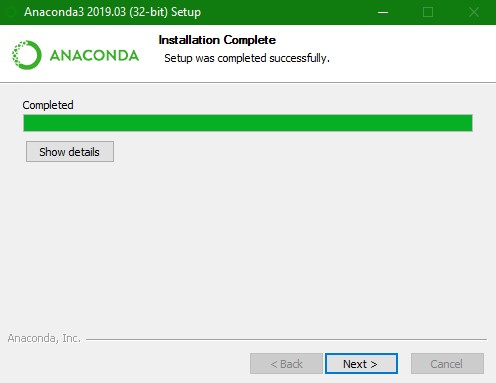
\includegraphics[scale=0.6]{gambar/7.jpg}
    \caption{\textit{Instalasi selesai}}
    \label{Figure7}
\end{figure}

\item Saat instalasi selesai klik \textit{next}


\begin{figure}[!htbp]
    \centering
    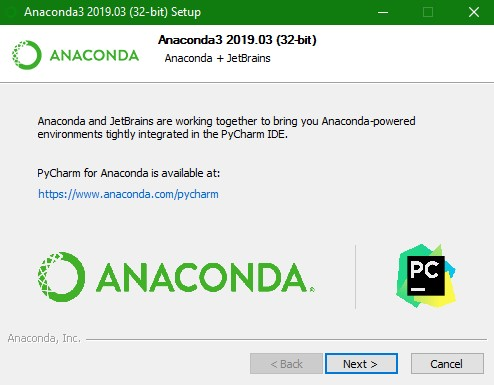
\includegraphics[scale=0.6]{gambar/8.jpg}
    \caption{\textit{Selesai klik next}}
    \label{Figure8}
\end{figure}

\item Selanjutnya klik \textit{next} 


\begin{figure}[!htbp]
    \centering
    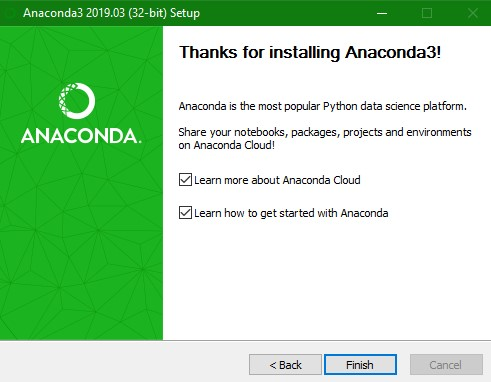
\includegraphics[scale=0.6]{gambar/9.jpg}
    \caption{\textit{Proses akhir}}
    \label{Figure9}
\end{figure}

\item Klik \textit{finish} saat sudah selesai instalasi

 
\end{enumerate}
\subsection{instalasi pip}
\Cara menginstal pip langkah pertama yaitu buka cmd\\
lalu ketikan di cmd : conda install -c anaconda pip lalu enter\\

\begin{figure}[!htbp]
    \centering
    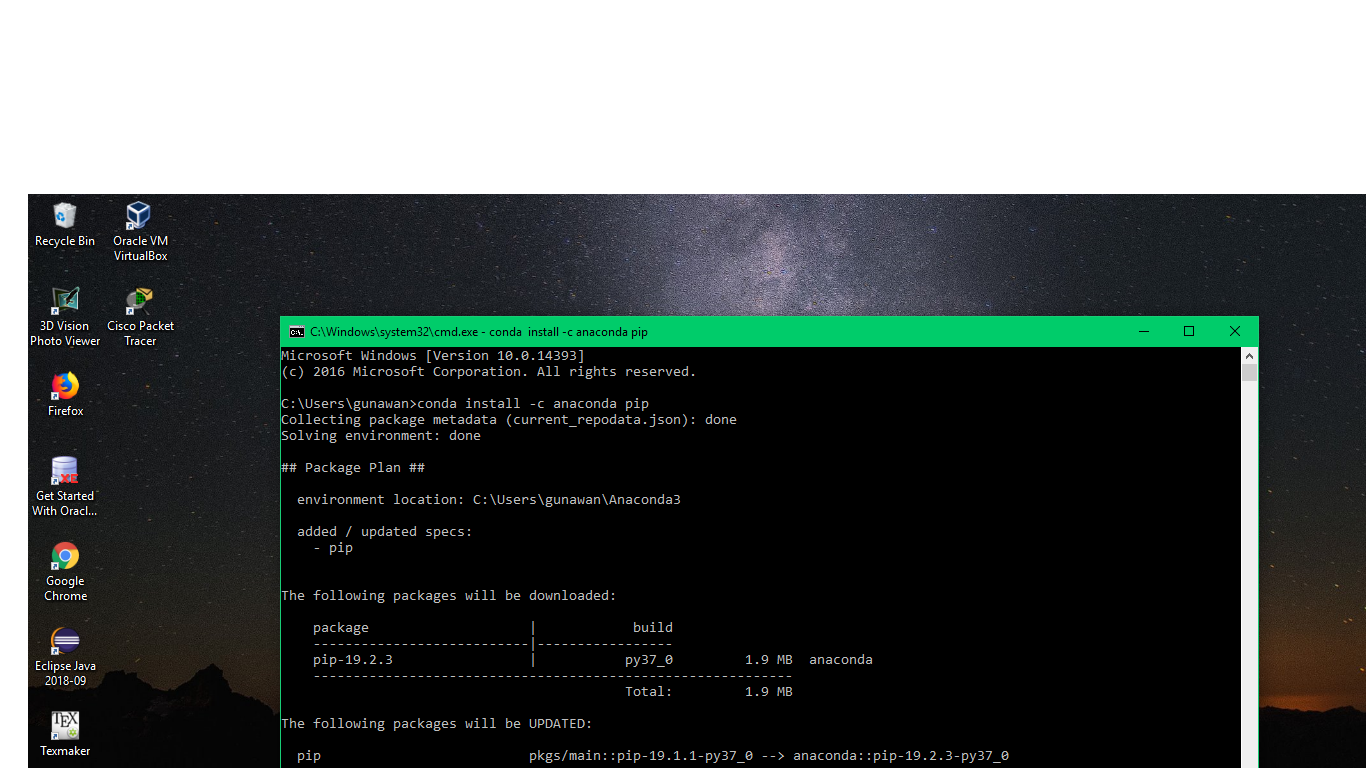
\includegraphics[scale=0.3]{gambar/Instal pip.png}
    \caption{\textit{install pip}}
    \label{Figur88e1}
\end{figure}

\par Lalu masukan huruf y pada pilihan ([y]/n) 

\begin{figure}[!htbp]
    \centering
    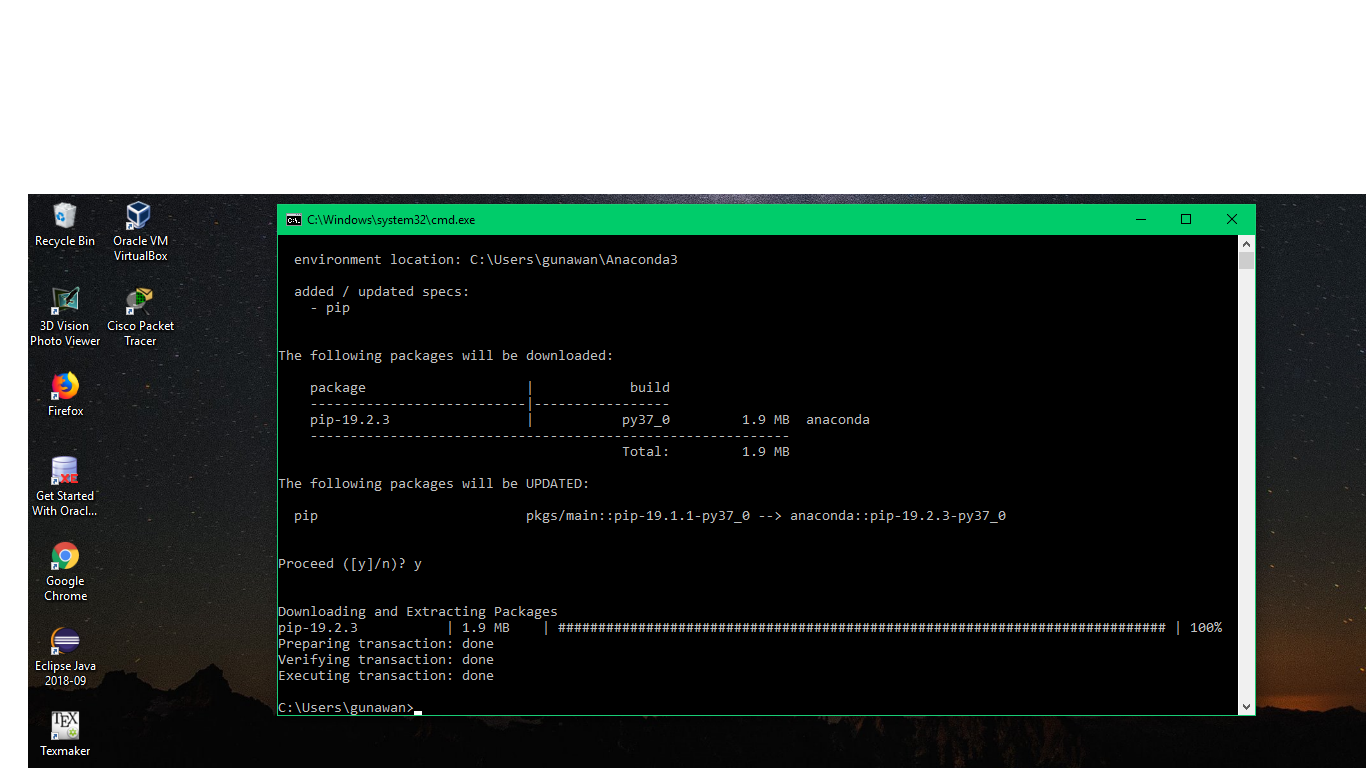
\includegraphics[scale=0.3]{gambar/Instal pip done.png}
    \caption{\textit{masukan huruf y}}
    \label{Figure1}
\end{figure}

\par Tunggu hingga Dowloading selesai

\subsection{Cara setting environment}
\par Caranya pertama kita buka File Explorer di Windows, kemudian klik kanan pada This PC untuk pengguna Windows 

\begin{figure}[!htbp]
    \centering
    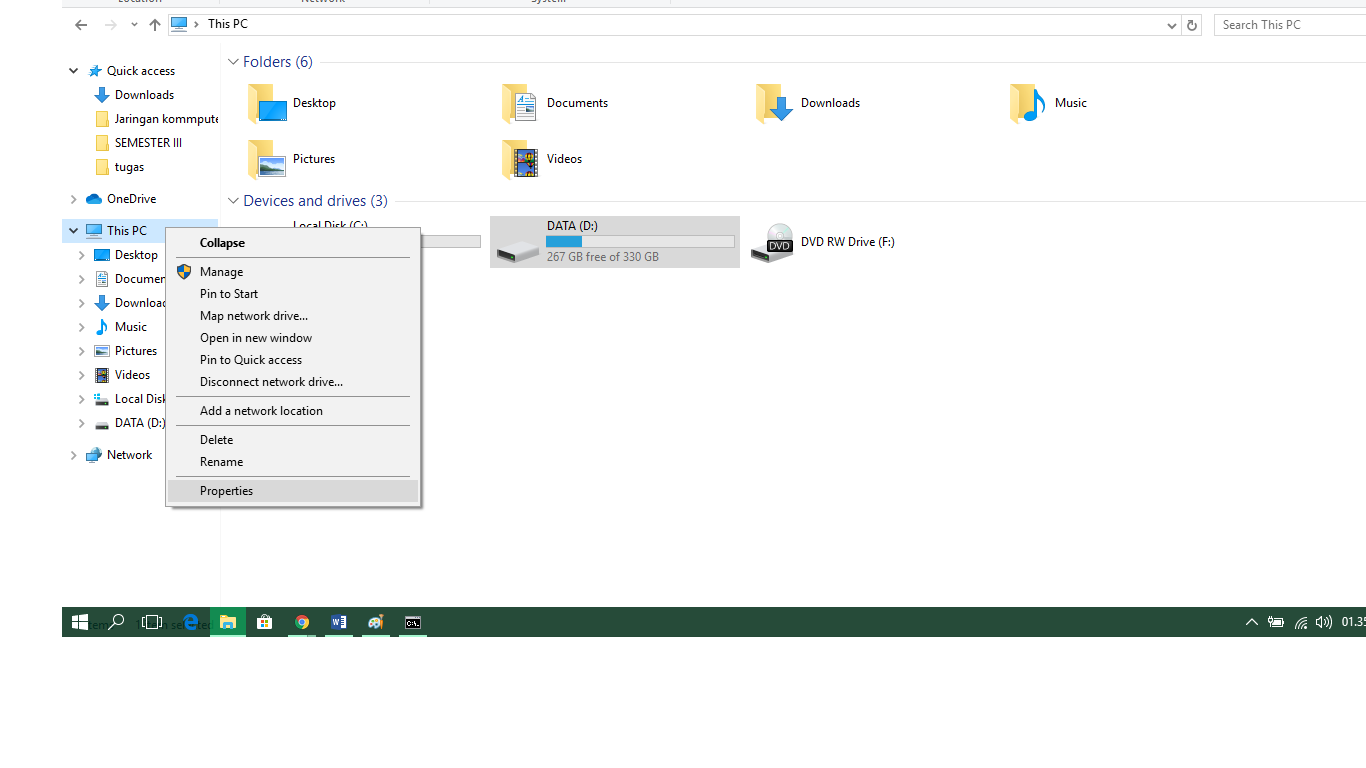
\includegraphics[scale=0.3]{gambar/cek ev.png}
    \caption{\textit{Setting environment}}
    \label{Figure1}
\end{figure}


\par Selanjutnya Pilih Advanced System Settings

\begin{figure}[!htbp]
    \centering
    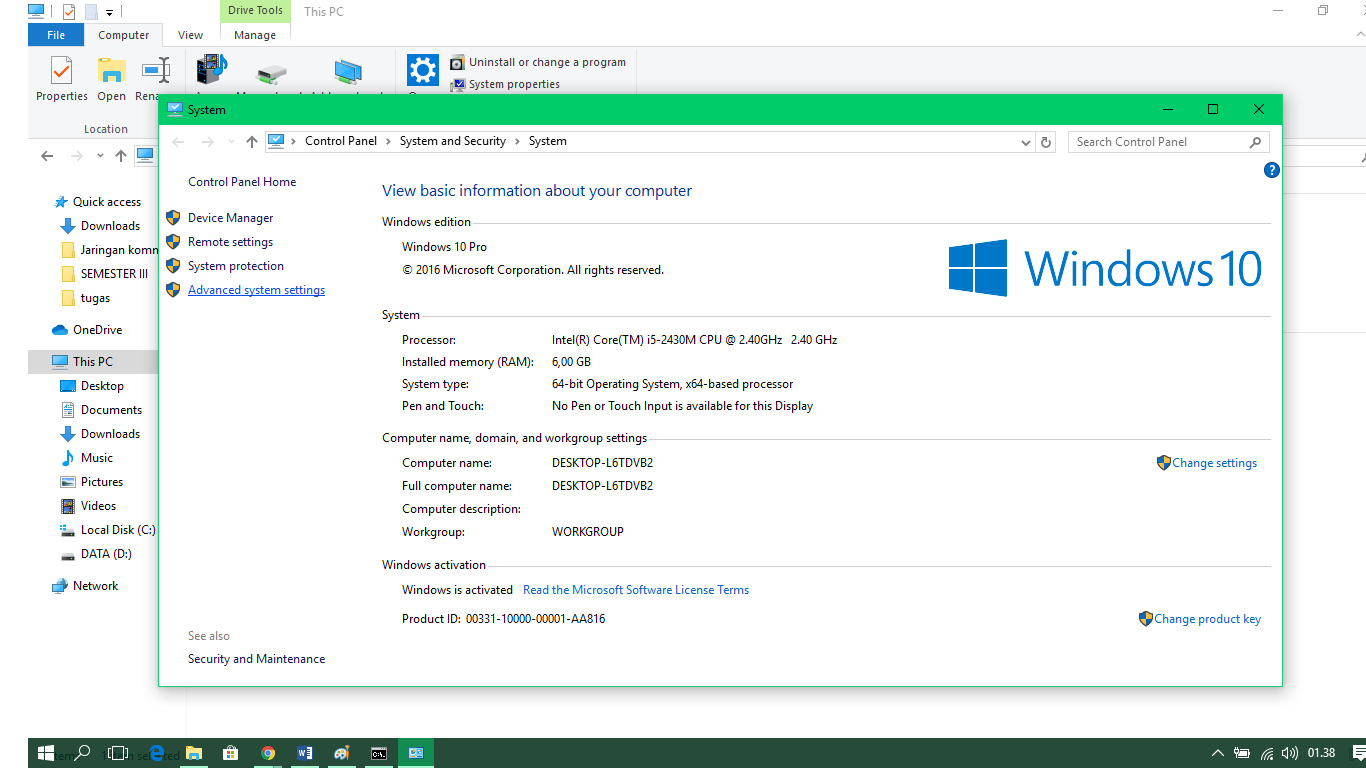
\includegraphics[scale=0.3]{gambar/cek ev1.png}
    \caption{\textit{Setting environment}}
    \label{Figure312}
\end{figure}

\par Pada System Properties, Pilih tab Advanced klik tombol Environment Variables

\begin{figure}[!htbp]
    \centering
    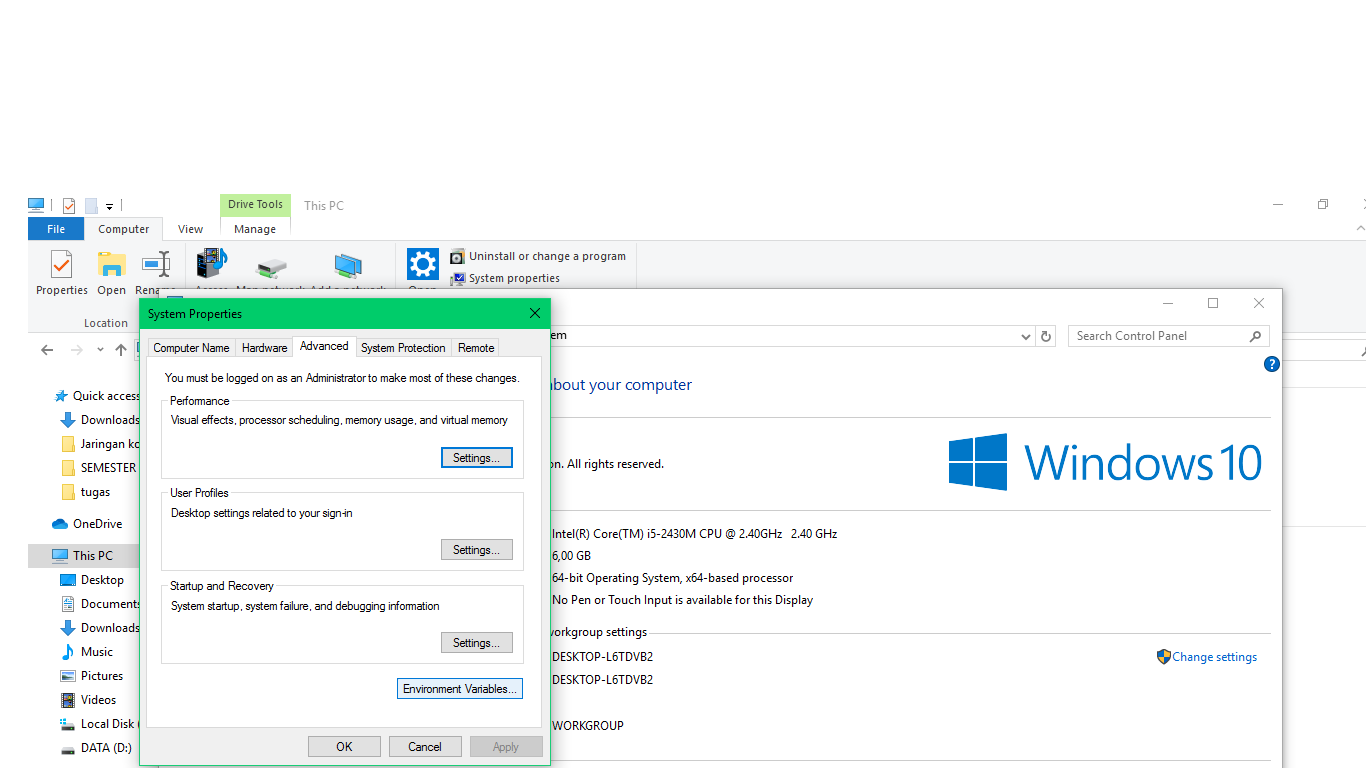
\includegraphics[scale=0.3]{gambar/cek ev2.png}
    \caption{\textit{Setting environment}}
    \label{Figure44412}
\end{figure}

\par Pada Environment Variables, kita akan memilliki/klik System Variables Path dan klik Edit 

\begin{figure}[!htbp]
    \centering
    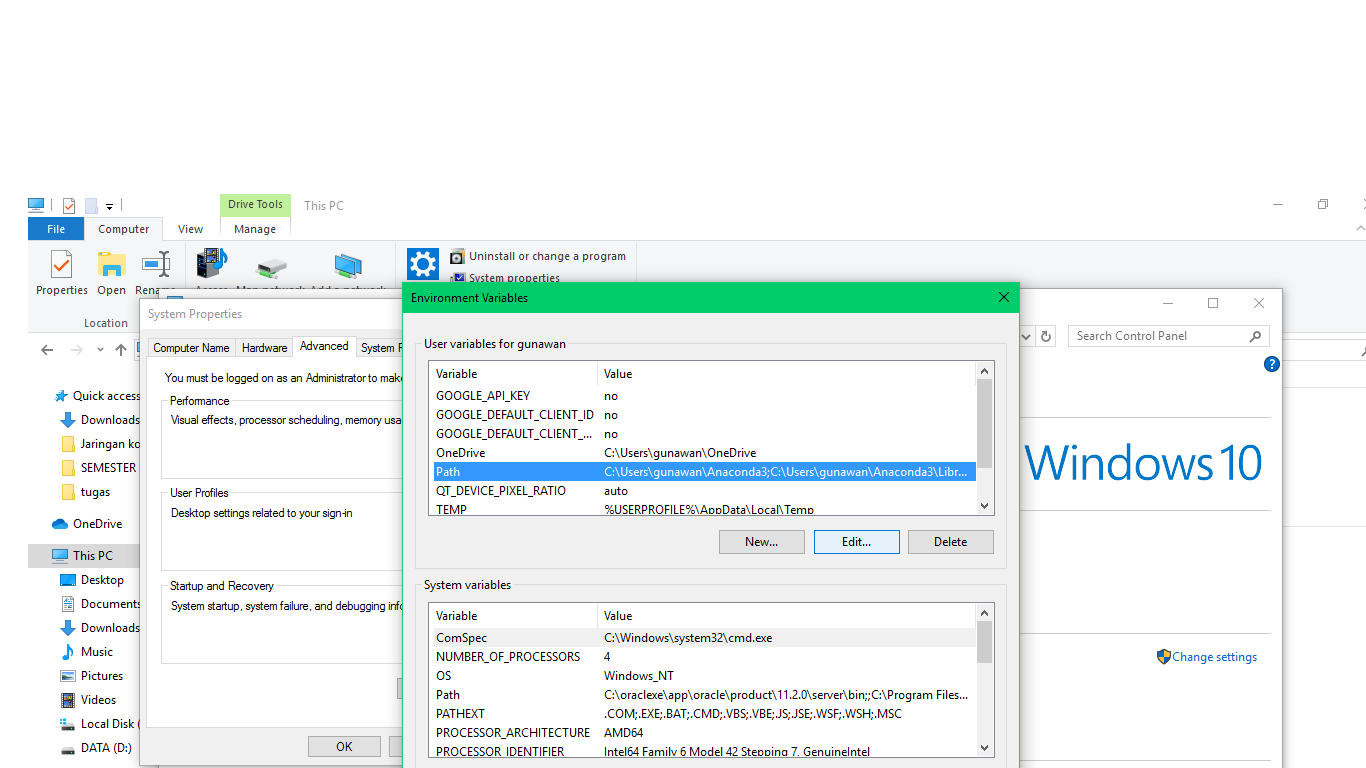
\includegraphics[scale=0.3]{gambar/cek ev3.png}
    \caption{\textit{Setting environment}}
    \label{Figure23512}
\end{figure}

\par Lalu pilih settingan yang ingin kita gunakan

\begin{figure}[!htbp]
    \centering
    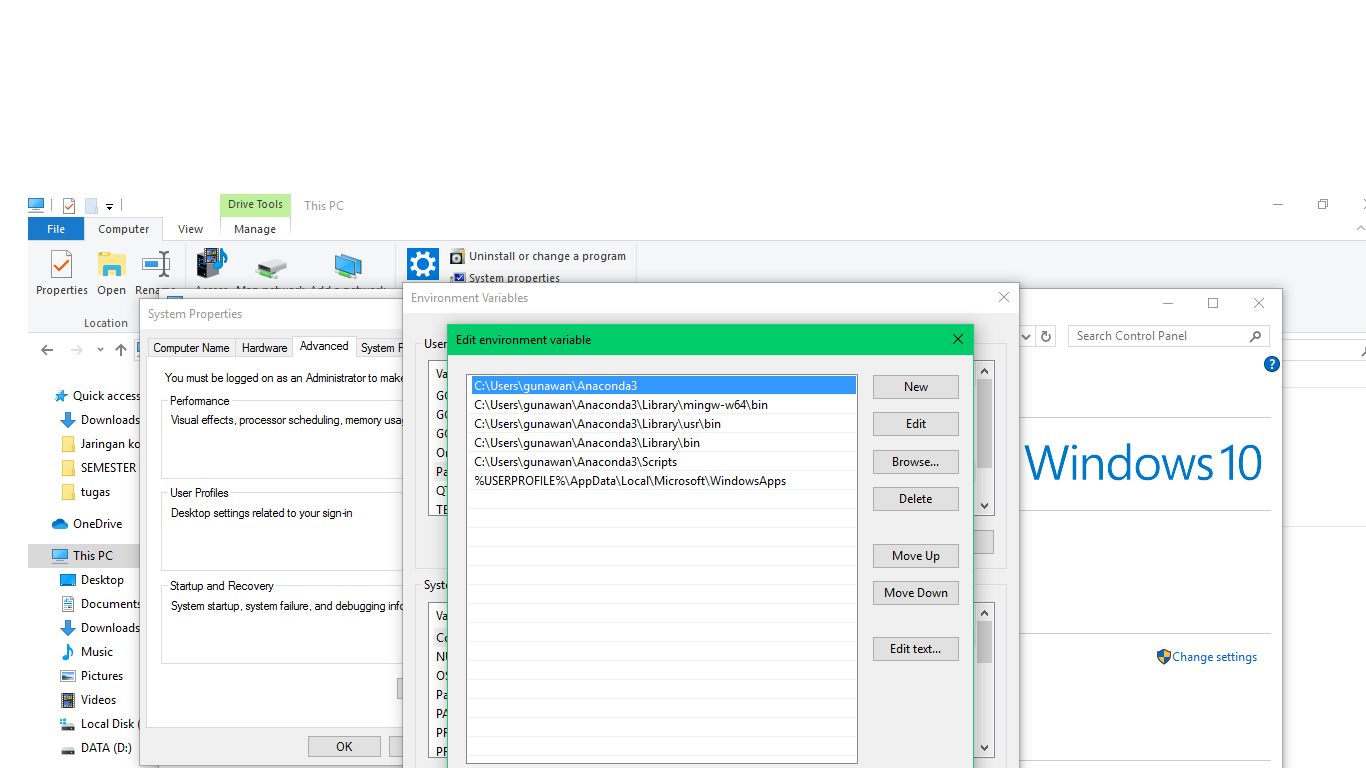
\includegraphics[scale=0.3]{gambar/cek ev4.png}
    \caption{\textit{Setting environment}}
    \label{Figure12}
\end{figure}

\par klik ok 

\subsection{Mencoba enterpreter/cli melalui terminal atau cmd windows}

\par Buka cmd lalu ketik python di dalam cmd,tekan enter lalu ketikkan print ("Hello word") lalu enter lalu akan keluar "Hello word"

\begin{figure}[!htbp]
    \centering
    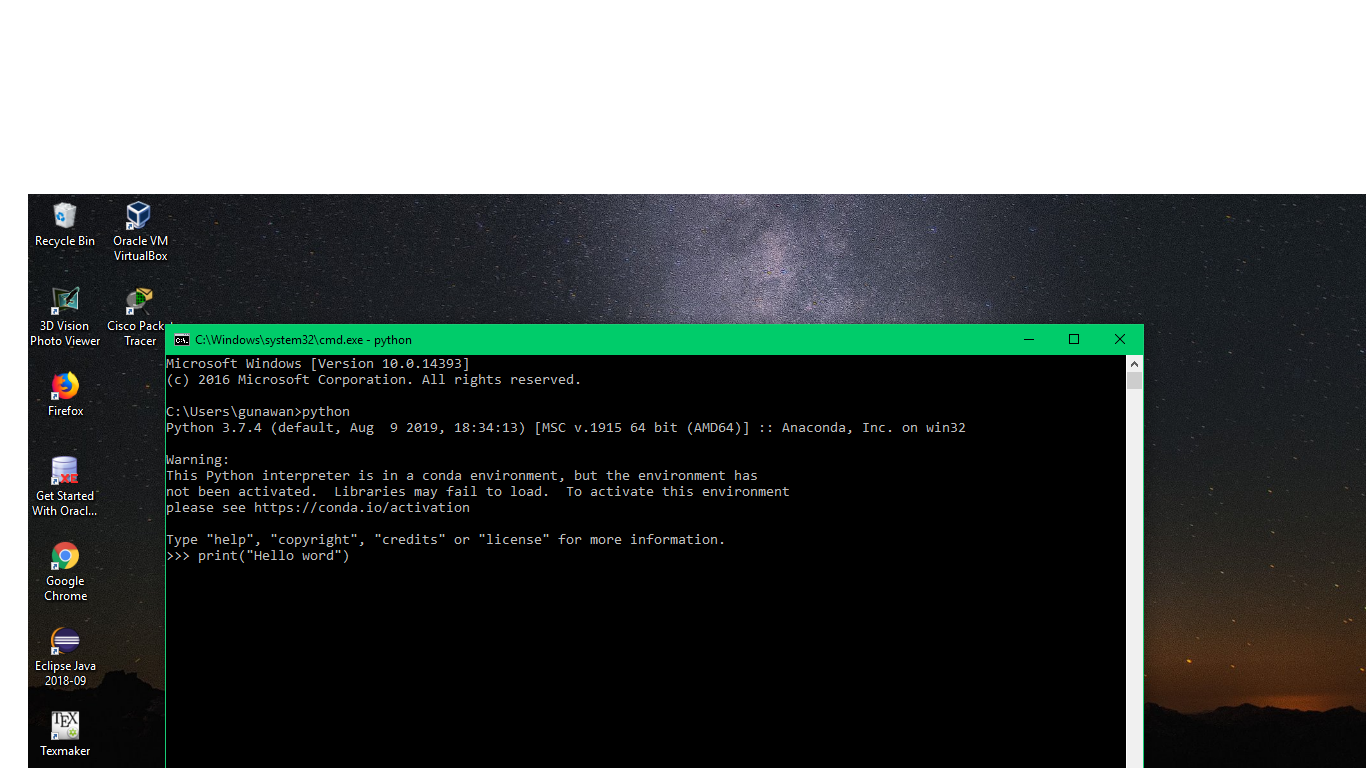
\includegraphics[scale=0.3]{gambar/cli.png}
    \caption{\textit{entrepreter/cli}}
    \label{Figure1}
\end{figure}

\subsection{Menjalankan dan mengupdate anaconda dan spyder}

\par   Buka cmd untuk mengupdate ketikan conda install -c anaconda python\\
lalu untuk mengupdate spyder ketikan conda install -c anaconda spyder


\begin{figure}[!htbp]
    \centering
    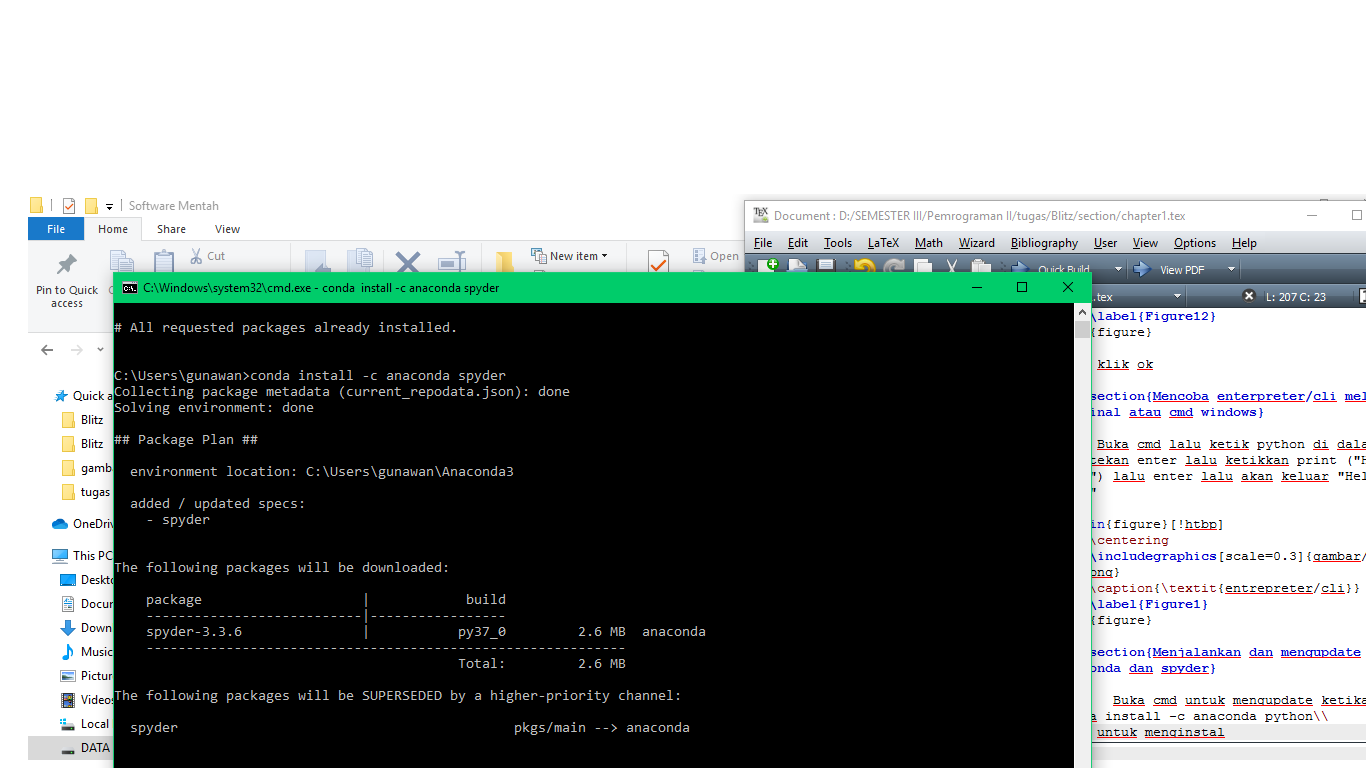
\includegraphics[scale=0.3]{gambar/spydernew.png}
    \caption{\textit{update anaconda dan spyder}}
    \label{Figure3331}
\end{figure}


\subsection{Cara menjalankan Script Hello word di spyder}

\par Buka aplikasi spyder ketikan print ("Hello word") lalu run atau tekan F5

\begin{figure}[!htbp]
    \centering
    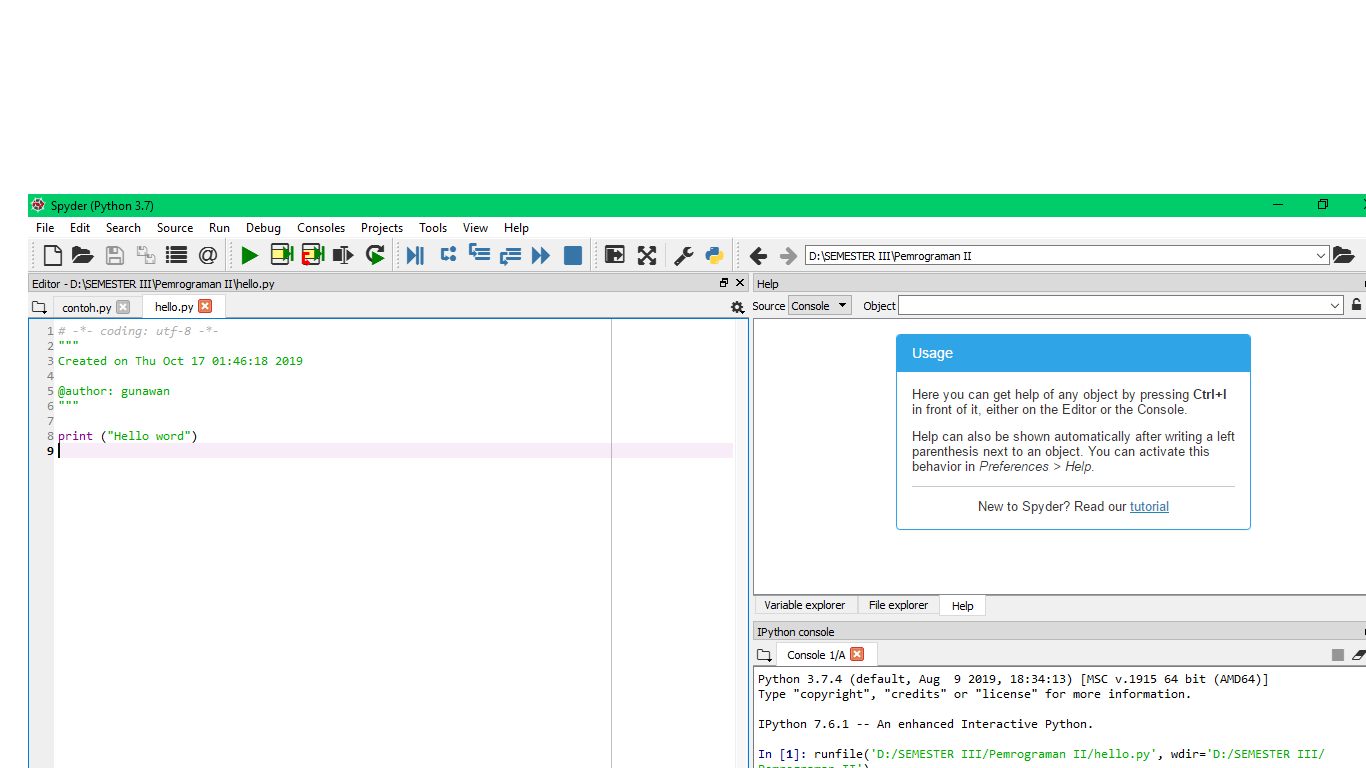
\includegraphics[scale=0.3]{gambar/hello.png}
    \caption{\textit{Hello word}}
    \label{Figure1}
\end{figure}

\subsection{Cara menjalankan Scirpt otomatis login aplikasi akademik dengan library selenium dan inputan user }

\begin{figure}[!htbp]
    \centering
    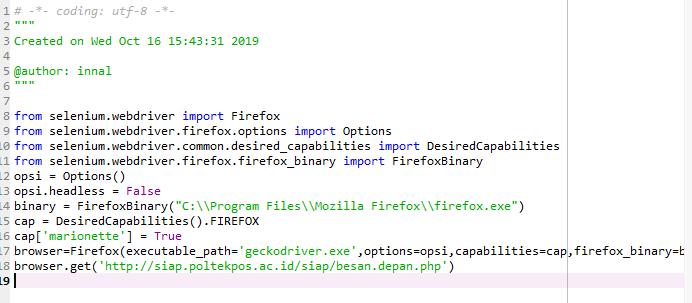
\includegraphics[scale=0.3]{gambar/code.png}
    \caption{\textit{Script}}
    \label{Figure1}
\end{figure}

\subsection{Cara pemakaian variable explorer di spyder}

\par Langkah pertama yaitu buka spyder lalu setelah kita buka spyder ketikan kodingan seperti contoh ini : nama = ("Bambang") print ("Siapa nama kamu",nama") \\
lalu run atau tekan F5, nanti akan terlihat dikolom kana bawah hasil dari script , lalu setelah itu untuk melihat variable explorer bisa dilihat dikolom atas seperti di gambar 

\begin{figure}[!htbp]
    \centering
    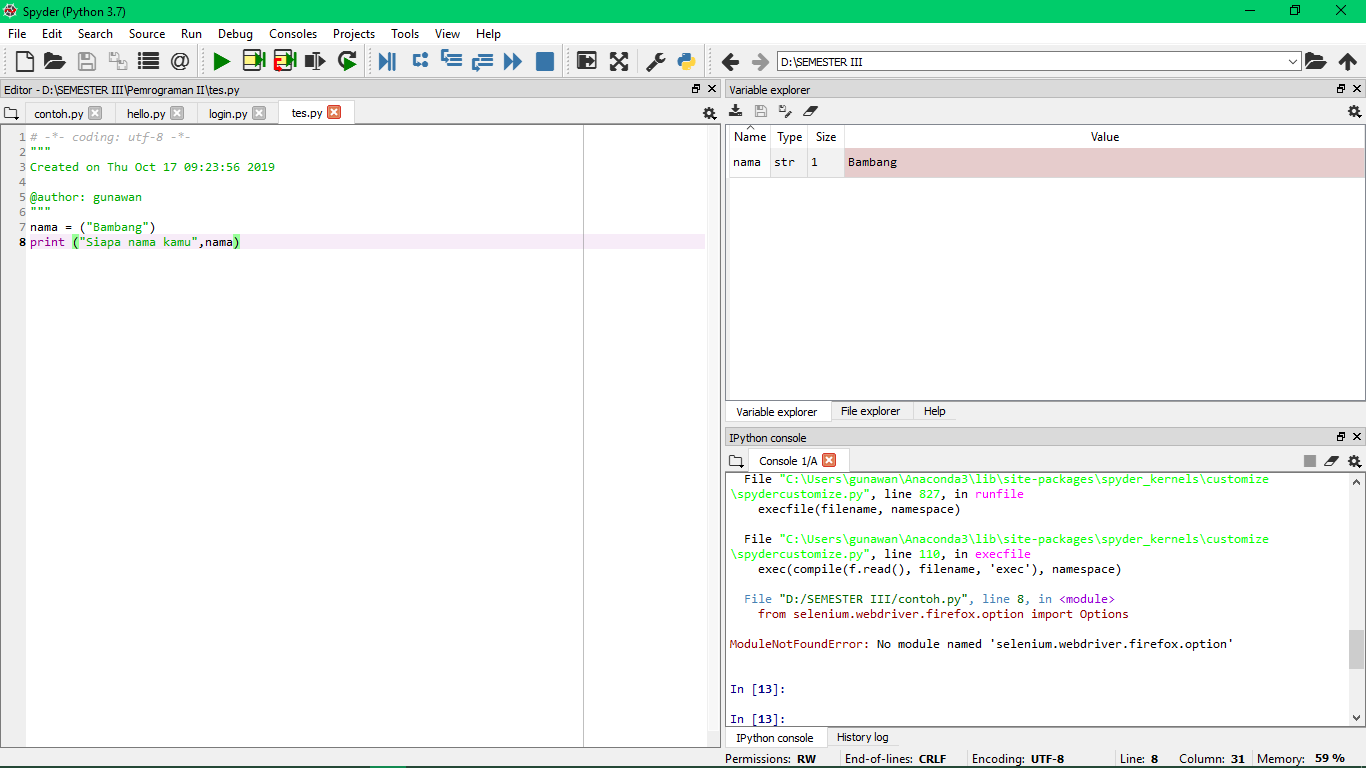
\includegraphics[scale=0.3]{gambar/tess.png}
    \caption{\textit{Variable}}
    \label{Figure1}
\end{figure}

\section{Identasi}
\subsection{Penjelasan identasi}
identasi adalah bagian paragraf yang menjorok ke dalam pada baris - baris paragraf, penulisan kode python tidak memakai curly bracket "{}" sehingga cara memebedakan blok program digunakan identasi
jenis error identasu fungsi if memerlukan indentasi untuk membedakan blok kode solusinya yaitu menambahkan indentasi sebelum fungi print.\\
Error akan terlihat di IPython console. Cara menyelesaikan error tersebut dengan cara mengatur spasi sesuai kebutuhan, jika bagian code tersebut bukan merupakan fungsi maka tidak boleh diberi spasi sedangkan jika merupakan bagian dari isi fungsi, maka harus diberi spasi 